
\chapter{Introduction} \label{chap:intro}

The indoor localization of people has a large range of possible applications. It can be used for navigation in unknown environments, such as firefighters in an emergency situation or personal navigation through large public buildings \cite{Correa2017, Jackermeier2018}. Another application is the tracking of individuals, such as within elderly homes or workers in a factory setting \cite{Correa2017}. \par

Human indoor localization is an ongoing research field where there is yet a solution to be found that is widely accepted as the state of the art \cite{Davidson2017}. Unfortunately, the well-known solution for outdoor localization, the Global Positioning System (GPS) \cite{Jackermeier2018}, cannot be applied reliably in an indoor environment. GPS is a constellation of satellites circling the globe, emitting radio signals at specific frequencies. Once received, these signals can be used to triangulate a position. However, radio waves have difficulty in crossing solid structures reliably. Additionally, if a signal is received indoors, it may have been rebounded off of radio reflective surfaces, causing erroneous positioning estimates \cite{Jackermeier2018}. \par 

For any indoor localization method to be widely applicable, it is preferable that an indoor localization method provide accurate position estimations, is easily scalable, and has low system infrastructure cost \cite{Correa2017}.
In line with these applicability wishes, the smartphone has proven to be the perfect platform for implementation. It is an untethered device widely used in the developed world \cite{Correa2017}, containing many different sensors combined with computing and communication capabilities.
Creating a system that works well on this device will be crucial to launching indoor localization on a global scale \cite{Gu2019}. Focusing on this platform brings additional technical restrictions to what any eventual solution can use. This includes robustness in carrying modes and computational requirements.  For example, the continuous use of a camera is not beneficial for battery life, limiting the use of this method \cite{Yang2014, Solin2018a}. Due to the advantages that smartphones bring, they have been used often in indoor localization research \cite{Jackermeier2018,Correa2017,Yang2014, Qian2013}. \par 

Within the research field of indoor localization, the approaches are either infrastructure dependent or infrastructure independent, both using sensors on the target. Combined solutions have attempted to use the advantages of each to improve performance \cite{Gu2019, Correa2017}. The infrastructure \textit{dependent} methods imitate the GPS setup on a local scale. They often replace the GPS constellation with other signal-producing devices available within the indoor environment. Some of these systems, such as wireless fidelity(Wifi) and Bluetooth, are detectable through smartphone sensors, while wireless sensor networks (WSN), and ultra-wideband (UWB) require dedicated devices or attachments \cite{Wu2019,Jackermeier2018,Davidson2017}. For many of these solutions, detailed information on the position of the external signal-producing devices may be needed for estimation, including a signal strength map or device location \cite{Jackermeier2018,Shang2015}. This information may not be easily available. Furthermore, these solutions naturally only work in buildings with the installed equipment. This requires either that they are already present or some initial investment and setup is made. In some cases, this can not be expected. For example within subway systems, where legal or investment issues and potential vandalism can be a hindrance \cite{Torok2014}. \par
%
% Position estimation using these systems can be range based, leveraging signal time of arrival, signal angle or received signal strength. They can also be range free using proximity and fingerprinting to estimate position \cite{Correa2017, Tariq2017}

Infrastructure \textit{independent} positioning solutions do not need to receive signals from external devices. Since no external infrastructure is required, these methods can have low infrastructure cost. Many such methods make use of cameras or \ac{IMU} sensors placed on the target (sensors often found in smartphones). Camera-based systems use unique visual features tracked in subsequent frames to determine displacement \cite{Gu2019}. With such an approach, privacy concerns, computing complexity, and device placement need to be considered \cite{Gu2019}. Inertial sensor-based methods use sensors that measure linear acceleration and angular velocity. They are \ac{MEMS},  consisting of triaxial orthogonal accelerometers and gyroscopes, and can include a triaxial magnetometer \cite{Yang2014}. These sensors are relatively small, cheap, and have low power consumption \cite{Olsson2016}. Low power consumption allows for long periods of use, and therefore potential long-term localization. The methods that use these sensor for location estimation are known as \ac{PDR}. \par

The combination of a smartphone with a wearable device is an important development in indoor localization technology. While the smartphone market has matured, the market for wearable devices has been growing steadily \cite{jung2016consumer}, with the smartwatch being the most prominent. These devices offer similar sensors and capabilities as smartphones, with the same advantages and disadvantages. One form of information that they can provide is the detection of interactions with the indoor environment, also known as activity recognition. These interactions may not be easily detectable through smartphone sensors alone \cite{Shoaib2015}. This can help with localization since some indoor interactions can be position-dependent. Examples include interacting with doors, stairs, and furniture. By knowing the location of these structures within the indoor environment, a position measurement is available if a relevant interaction is detected. This information can be combined with smartphone based systems to potentially improve indoor localization.

\section{Thesis Contributions}

In this thesis I am further exploring the combined technology of smartphones and wearable device by investigating how IMU sensors in a smartwatch can be used to improve smartphone IMU-based indoor localization. I will present the different \ac{PDR} methods available and research that combines them with some form of activity recognition. Afterwards a research gap will be highlighted, and a research question will be defined. With this research gap in mind, I will be focusing on a specific \ac{PDR} method, namely Step and Heading System. This will be combined with different drift reduction techniques, including a map based particle filter and landmark detection through activity recognition. The reasoning for these choices and how they work will be present in  \cref{sec:relevant_research}. A proof of concept will be designed and tested in a realistic environment. Results will be summarized and analyzed, indicating the performance and  limitations of the approach.

\section{Pedestrian Dead Reckoning }
\label{sec:relevant_research}
The person focused indoor localization technique that uses MEMS IMU sensors is called inertial Pedestrian Dead Reckoning (PDR). Dead reckoning indicates that the output of the system will be the relative position change from a starting point \cite{Yu2018}. Within PDR there are two methods, namely Inertial Navigation Systems (INSs) and Step and Heading Systems (SHSs). The INS mechanism integrates the IMU signals directly and is the implementation used most often within research \cite{Diez2018b}. SHS is based on integrating the displacement vectors associated with each step taken during pedestrian locomotion \cite{Davidson2017}.  \par

\subsection{Inertial Navigation System}
\label{sec:INS}
\begin{figure}[H]
	\centering
	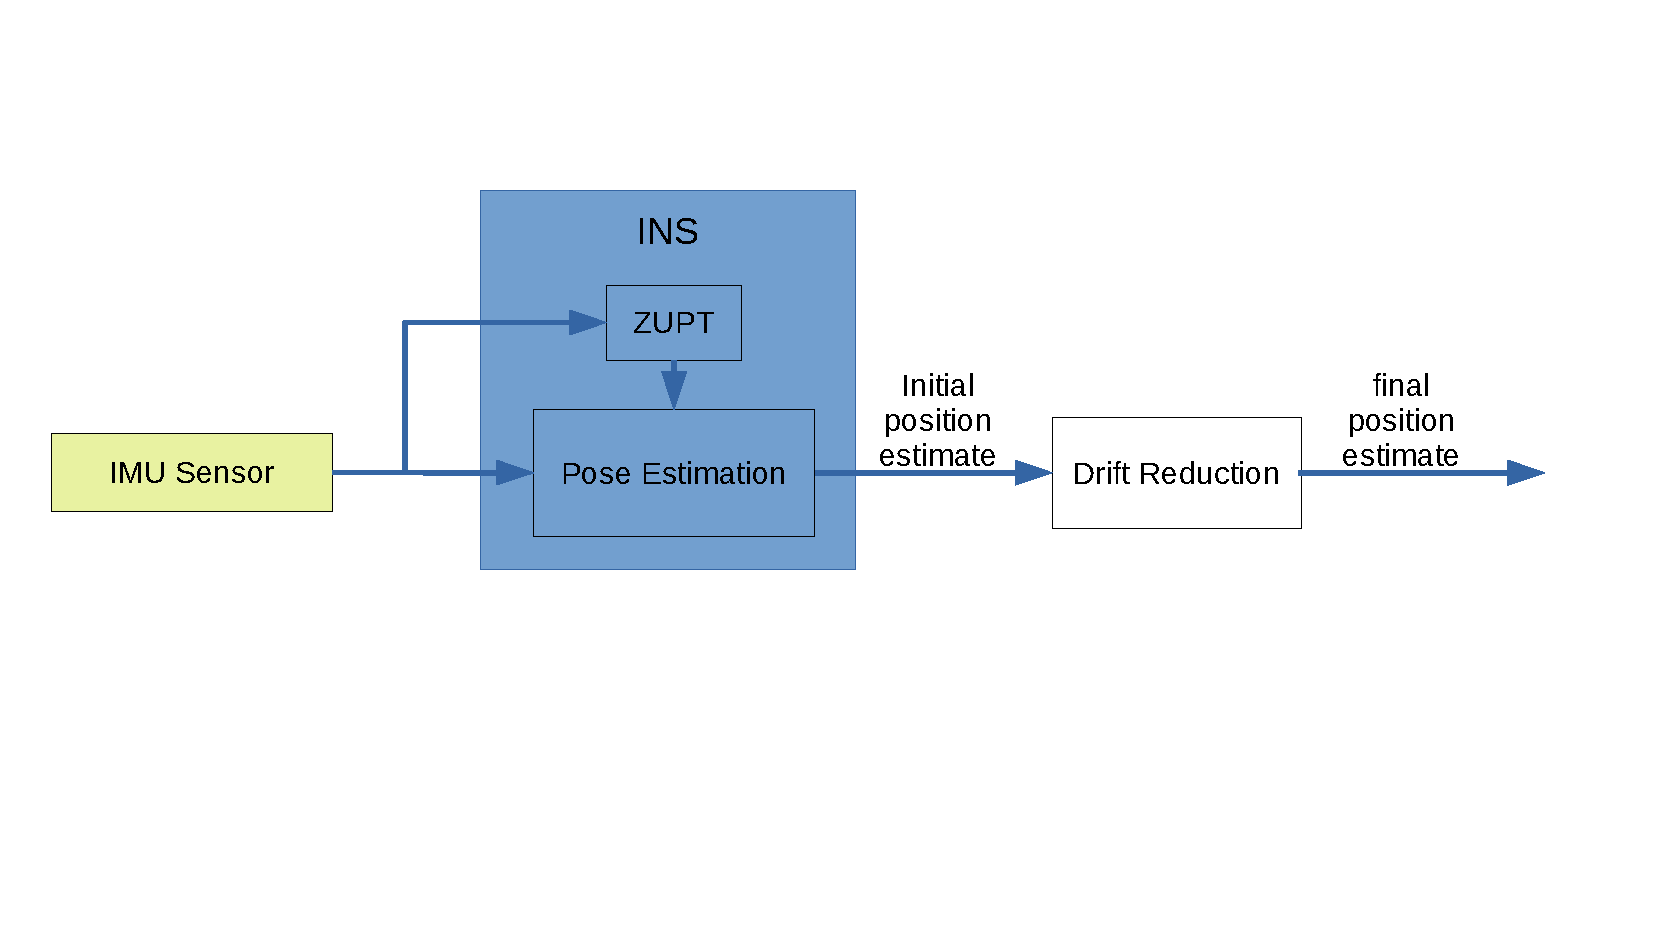
\includegraphics[trim=20 140 290 80, clip, width=0.8\linewidth]{images/INS_diagram}
	\caption{\ac{INS} pedestrian dead reckoning}
	\label{fig:ins_diagram}
\end{figure}
An Inertial Navigation System, as seen in \cref{fig:ins_diagram}, estimates pose, consisting of orientation and position, using sensor fusion algorithms. These methods are directly applied to the signals generated by MEMS IMU sensors \cite{Wu2019}. Examples of sensor fusion algorithms are the Extended Kalman Filter (EKF) and Complementary Filter (CF) \cite{Kok2017}. Sensor fusion algorithms can estimate position and orientation by integrating acceleration twice and integrating angular velocity once, respectively. This integration, in combination with the effects of noise and bias found in MEMS IMU, causes estimation errors to grow cubically with time for INS \cite{Harle2013}. \par

A technique frequently used to compensate for the built-up error in INS is zero velocity update (ZUPT) and zero angular update (ZARU) \cite{Harle2013}. It utilizes the ability to detect time periods in which the sensor is stationary during locomotion. Once detected, ZUPT uses the assumption that speed and angular velocity are zero at that time moment \cite{Wu2019,Harle2013}. this a form of pseudo-measurement. This is because the stationary phase is detected, with zero angular and linear velocity being implied by the assumption, which is not an actual measurement. Comparing the assumption with the output of the sensor fusion algorithm, an error can be calculated and used to compensate for the sensor fusion estimate. This process is generally known as a measurement update and can occur every time a stationary period is detected.  Through this form of measurement update the error grows linearly with number of steps \cite{foxlin2005pedestrian}.\par

Detecting brief stationary time periods in pedestrian IMU data is done easiest when the sensor is placed on the foot \cite{Diez2018,Davidson2017}. This is because a stationary period is much more pronounced in accelerometer data when the sensor is placed there \cite{Yu2019,Wu2019}.  When walking, a foot periodically returns to an actual stationary state and stays there for a brief period of time, approximately 0.1 to 0.3 seconds \cite{Ren2016a}. This has lead to most \ac{INS} research being foot-sensor based \cite{Diez2018,Wu2019}. A recent deviation from this trend, \citet{Solin2018a} overcome this preference for a foot-based system with a combination of several different pseudo measurements, loop closure, and position fixes, opening up new possibilities for implementing INS in non foot based use cases.\\
%The highest accuracy in PDR has been reached with INS in combination with ZUPT \cite{Hardegger2012}.

% Considering this, a focus will be put on implementing a SHS with the potential to handle different carrying modes.
\subsection{Step and Heading System}
\label{sec:rw-SHS}
\begin{figure}[H]
	\centering
	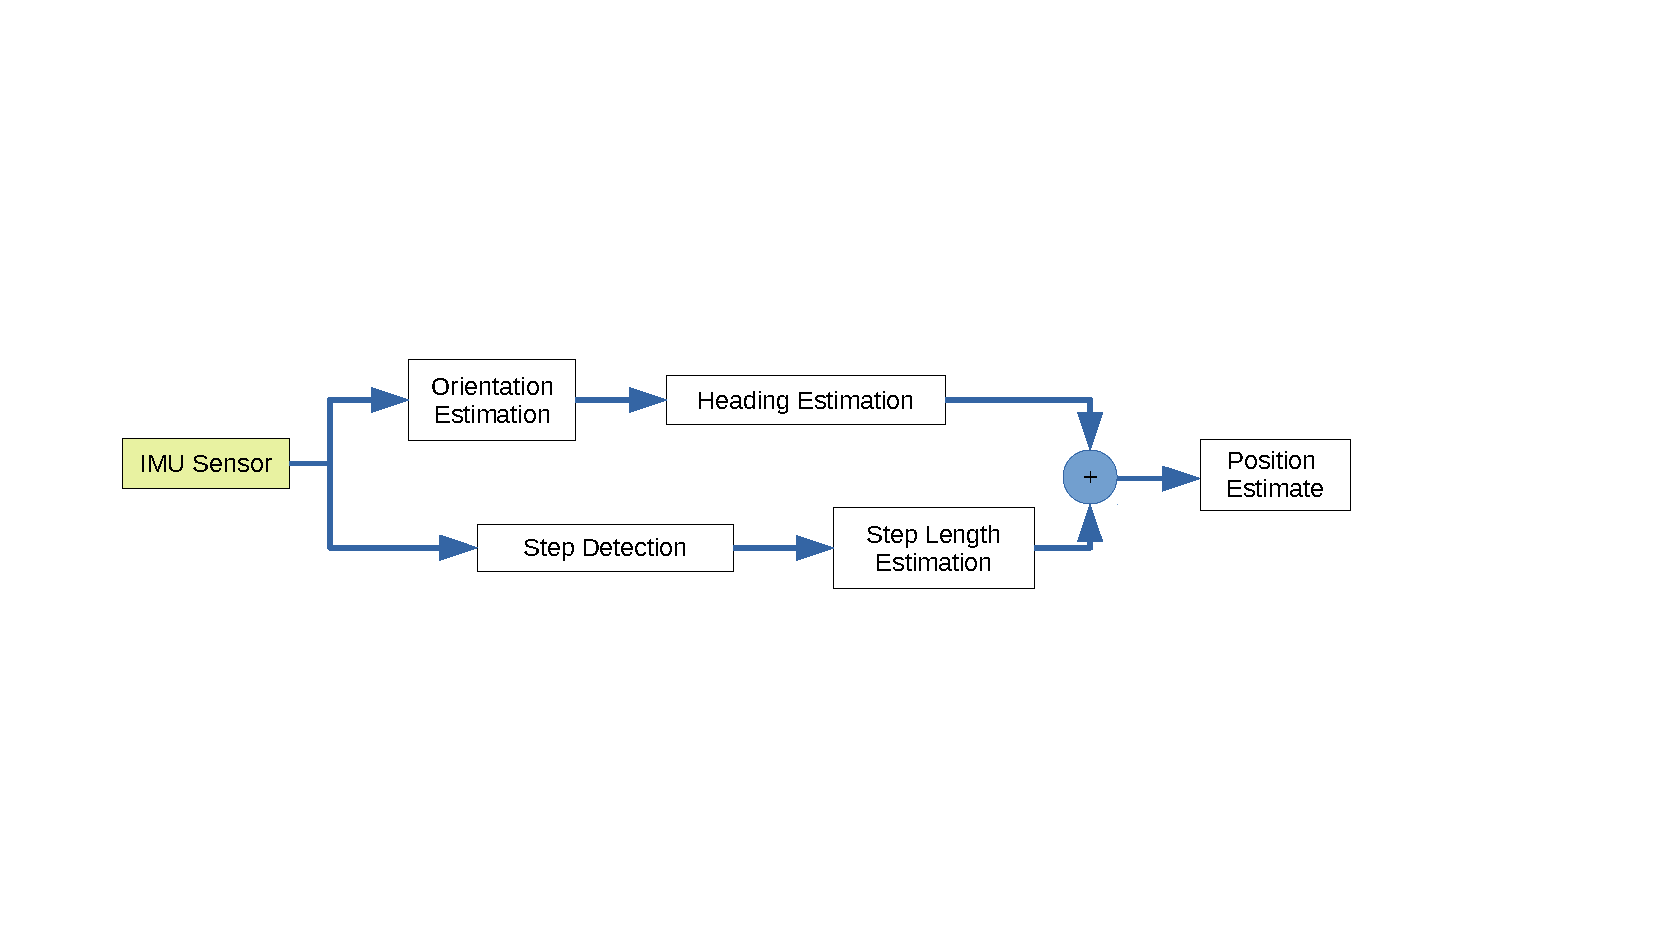
\includegraphics[trim=40 120 180 80, clip,width=\linewidth]{images/shs_diagram}
	\caption{\ac{SHS} pedestrian dead reckoning}
	\label{fig:shs_diagram}
\end{figure}
A step and heading system, as shown in \cref{fig:shs_diagram}, is a form of dead reckoning that detects steps, estimates step length, and the heading in which the pedestrian is moving. This position estimation can be represented by \cite{MunozDiaz2019}
\begin{equation}
	\label{eq:SHS_dynamic_model}
	\left(\begin{array}{l}
		x_t \\
		y_t
	\end{array}\right) 
	=
	\left(\begin{array}{l}
		x_{t-1} \\
		y_{t-1}
	\end{array}\right) 
	+l_{t} \left(\begin{array}{l}
		\cos \left(\theta_{t}\right) \\
		\sin \left(\theta_{t}\right)
	\end{array}\right)
\end{equation}

where $x_{t}$  and  $y_{t}$ represent the position in the $x$-axis and $y$-axis at time  $t$, respectively. $l_{t}$ stands for the step length, while $\theta_{t}$ is the step heading of the pedestrian at time $t$.
Similarly to INS with ZUPT measurement updates, SHS position error is proportional to the number of steps taken. The largest difference is that this error growth does not have a preference of using foot-based sensors, allowing for other sensor placements \cite{Diez2018b}. However, other of sources of error can be introduced due to errors in the detection of steps and their length estimation.  Since other sensor placements are possible, SHS is the PDR technique often used with smartphones as the base for sensing [\qn]. 

%This indicates that this technique is appropriate for further investigation in answering the thesis research questions.\\

%This method can be combined with a particle filter \cite{Koivisto2016, Jackermeier2018}. This allows for more constraints, consequently requiring less particles for localization.
\section{Drift Reduction through Landmark Detection}
PDR methods alone accumulate error with time and are therefore not ideal for long-term pedestrian tracking \cite{Hardegger2012}. Drift reduction methods can be used to try and compensate for this error \cite{MunozDiaz2019a}.  These methods use additional information to restrict the possibilities in which the position estimate can be. One approach is by complement the solution with the infrastructure dependent solutions that require external signal generation \cite{Gu2019}. Another source of information is spatial context \cite{Gu2019}. This includes maps, spatial models and landmarks. A map describes the indoor layout of building, often in the form of of a floor plan \cite{Gu2019}. Using maps assumptions or simplification to restrict the movement. Examples include restricting the movement to be parallel to the outer walls of a building \cite{Abdulrahim2011}. Another is representing the indoor environment as a set of links and nodes, along which the position estimate can move \cite{Davidson2017,Jackermeier2018} 
One approach to drift reduction is through the use of landmark detection. Landmarks are locations with a unique footprint detectable in sensor data. When the user visits a landmark and this is detected, the location of the landmark can be used to calibrate the position estimate of the user, hence compensating drift \cite{Diaz2017}. In addition to drift reduction by position comparison, landmark detection can also be used in determining the user specific parameters of \ac{SHS} online, such as step length estimation parameters \cite{Gu2019,Shang2015}.  Depending on the sensors available, different landmarks become detectable. Examples of landmarks are doors and stairs \cite{Diaz2017,Gu2019,Torok2014}, but also unique magnetic footprints \cite{MunozDiaz2019}, and electromagentic signal footprints \cite{Gu2019}. Some landmarks can be easily determined beforehand, through the use of available building blueprints \cite{Gu2019}. Others can be detected online \cite{Hardegger2012, Hardegger2016}, not requiring a map representation to be available beforehand, using technique such as \ac{SLAM}. 

One form of landmark detection can be done through activity recognition. \\
\textcolor{cyan}{above section can be smoother} \\ \newline
\textcolor{cyan}{ I need to refer to the use of particle filters and that for PDR their use is two fold, landmark detection and absolute position estimate}

\subsection{Activity Recognition}
Activity recognition is large research field in which methods span a broad range of complexity, from simple thresholding to the use of deep learning techniques such as neural networks and its many variations \cite{Lima2019}. Even the subset of activity recognition that use IMU sensors does not decrease the amount of possibilities significantly.

%TODO add drear as activity recognition

The choice for a particular activity recognition method is often a trade-off between performance and computational complexity \cite{Bulling2014}. Considering the scope of this thesis, certain constraints can be applied, such as that the system should be able to function on a smartphone and must use comparable sensors to those found in such devices, thus MEMS IMUs. \citet{Shoaib2015} have performed an extensive survey that focuses on the online activity recognition solely using mobile phone sensors and onboard processing. Other metrics such as resource consumption were also presented. 30 papers were found to meet the requirements of the review. Within the review they indicate that most commonly used classification methods include Decision Tree, support vector machine (SVM), K-nearest neighbor (KNN) and Naive Bayes, in descending order. A third of the papers were found to use decision trees. All but 6 of the papers had the training process occurring offline. The classification process takes the method generated offline, and uses it online to classify new activities. The authors refrain from listing any performance measures, such as accuracy or precision, since no direct comparison between the different methods is made. \citet{Ahmad2020} specifically focuses on seeing whether smartphone activity recognition techniques are also applicable to smartwatches, and what parameters, including classifiers, work best. Activities to recognize included walking, up-stairs, down-stairs, running, and jogging. Their results indicated that  Decision Trees, SVM and KNN had around 90 percent accuracy a minor difference. \citet{Shoaib2016} show that combining information from both a smartwatch and smartphone, complex human activity recognition is improved compared to when only a smart watch is used. 

\section{Pedestrian Dead Reckoning with Activity Recognition}

There is previous research that uses different forms of activity recognition to aid in localization. In some cases this can be a simple approach, such as applying a threshold on orientation change to determine if a corner has been turned or not. Once detected, corner definitions from map information is used to improve localization \cite{Gu2019,Jackermeier2018}. \par 
\citet{Hardegger2012} created ActionSLAM, which uses a foot mounted sensor to estimate displacement in combination with location-related actions to compensate any drift buildup. It does not require map information as it used \ac{SLAM}, to produce a map itteratively. In the case of ActionSLAM, the activity recognition was performed manually by annotating from video recordings. The paper indicates a tracking error between a ground truth and the calculated path to be around 1.3 meters. This research is augmented in \citet{Hardegger2016} have recognized the growing trend of wearable technology. They derived a method that used an INS based system in combination with activity recognition through template matching, particle filters, and SLAM to improve both activity recognition and localization. Examples of detected actions are opening a window, picking up a phone and opening a drawer. \par
A different approach was used by \citet{Grzonka2010}, who used a body suit composed of multiple IMU sensors to detect the opening and closing of doors as landmarks, also using a \ac{SLAM} approach for map generation. \citet{Torok2014} have developed DREAR, which is a hidden markov model to detect landmarks using a combination of map information and smartphone sensors, both inertial sensor and magnetometer, to detect when a person is sitting, walking, and taking an escalator.

\section{Research Question}

From previous research 
What effect can \ac{IMU} based activity recognition from a smartwatch have on a \ac{SHS}-\ac{PF} based \ac{PDR} approach with indoor localization?


\section{Thesis Outline}
%A solution with the potential to meeting the above requirements is Pedestrian Dead Reckoning (PDR), a technique where the displacement from an initial location is calculated for a pedestrian. This technique often uses inertial sensors, with different possible placements on the body \cite{Gu2019}. These sensors are \ac{MEMS}, and consist of triaxial orthogonal accelerometers and gyroscopes, and can include a triaxial magnetometer \cite{Yang2014}. These sensors are small, lightweight and cheap, and are found in almost all smartphone brands.
%While able to generate a position estimate for the pedestrian, position estimation drift is inevitable



%Dead reckoning (DR) presents an interesting, incremen­tal positioning modality for pedestrians, complementary to absolute positioning of modern mobile phones (GPS, WiFi, Bluetooth and others). Many location aware applications can profit from greater accuracy and indoor availability, that can be achieved by combining DR with absolute positioning modalities. While dead reckoning is limited for long-term use due to error accumulation, it can achieve high short- to mid-term accuracy, and can be used to gap non-availability phases ^citation from Dead Reckoning from the Pocket - An Experimental StudyUlrich Steinhoff* and Bernt Schiele*t
 
%Although global positioning system (GPS)–based outdoor localization is very common, indoor localization remains a challenge because GPS signals are unavailable indoors. Many indoor localization methods are based on wireless radio systems, such as Wi-Fi [2], radio-frequency identity [3], ultra-wideband [4], and Bluetooth [5]. These localization methods can be categorized into two types [6]: triangulation and fingerprinting. The former relies on installed expensive hardware, making it neither scalable nor universal. The latter requires pretraining, which is time-consuming. citation from A Robust Step Detection and Stride Length Estimation for Pedestrian Dead Reckoning Using a Smartphone 


%Repurposing smartphones for ubiquitous sensing is challenging due to their battery constraints and multi-purpose nature. We observed that each embedded sensor has a similar power draw if used individually, but using combinations of sensors costs significantly more (see Figure 1). Thus, we use solely the accelerometer (applicable even to early smartphones). Smartphones are not dedicated sensing devices and they suffer from dropped samples and significant jitter in signal timestamps. Moreover, their nonrigid attachment (they may be carried in front pockets; back pockets; shirt pockets; hands; bags and more) and freedom of motion violate many of the assumptions made in previous step detection work. citation from Brajdic and harle 2013 

%\section{Research Questions}
%\textcolor{red}{ATM I am not very sure on these research questions. I would like to discuss with you better options!}
%
%In order to tackle the subject, two main research questions can be defined, with further subquestions and explanation below them.
%
%\begin{itemize}
%	\item \textbf{How can indoor localization be achieved with realistic smartphone placement, while taking computation capabilities into account?}
%	\begin{itemize}
%		\item What indoor localization methods consider realistic smartphone carrying modes? 
%	\end{itemize}
%	\item\textbf{How can wearable devices improve indoor localization?}
%	\begin{itemize}
%		\item What information can be derived from wearable devices?
%	\end{itemize}
%\end{itemize}